% !TEX TS-program = pdflatex
% !TEX encoding = UTF-8 Unicode

% This is a simple template for a LaTeX document using the "article" class.
% See "book", "report", "letter" for other types of document.

\documentclass[11pt]{article} % use larger type; default would be 10pt

\usepackage[utf8]{inputenc} % set input encoding (not needed with XeLaTeX)

%%% Examples of Article customizations
% These packages are optional, depending whether you want the features they provide.
% See the LaTeX Companion or other references for full information.

%%% PAGE DIMENSIONS
\usepackage{geometry} % to change the page dimensions
\geometry{a4paper} % or letterpaper (US) or a5paper or....
%\geometry{margin=2in} % for example, change the margins to 2 inches all round
\geometry{left=2.75cm, right=2.75cm, top=3.5cm, bottom=4.5cm}
% \geometry{landscape} % set up the page for landscape
%   read geometry.pdf for detailed page layout information

\usepackage{graphicx} % support the \includegraphics command and options

% \usepackage[parfill]{parskip} % Activate to begin paragraphs with an empty line rather than an indent

%%% PACKAGES
\usepackage{booktabs} % for much better looking tables
\usepackage{array} % for better arrays (eg matrices) in maths
\usepackage{paralist} % very flexible & customisable lists (eg. enumerate/itemize, etc.)
\usepackage{verbatim} % adds environment for commenting out blocks of text & for better verbatim
\usepackage{subfig} % make it possible to include more than one captioned figure/table in a single float
% These packages are all incorporated in the memoir class to one degree or another...

%%% HEADERS & FOOTERS
\usepackage{fancyhdr} % This should be set AFTER setting up the page geometry
\pagestyle{fancy} % options: empty , plain , fancy
\renewcommand{\headrulewidth}{0pt} % customise the layout...
\lhead{}\chead{}\rhead{}
\lfoot{}\cfoot{\thepage}\rfoot{}

%%% SECTION TITLE APPEARANCE
\usepackage{sectsty}
\allsectionsfont{\sffamily\mdseries\upshape} % (See the fntguide.pdf for font help)
% (This matches ConTeXt defaults)

%%% ToC (table of contents) APPEARANCE
\usepackage[nottoc,notlof,notlot]{tocbibind} % Put the bibliography in the ToC
\usepackage[titles,subfigure]{tocloft} % Alter the style of the Table of Contents
\renewcommand{\cftsecfont}{\rmfamily\mdseries\upshape}
\renewcommand{\cftsecpagefont}{\rmfamily\mdseries\upshape} % No bold!

%%% BibTex packages (url for website references)
\usepackage[english]{babel}
\usepackage[numbers]{natbib}
% \usepackage{url}
% \usepackage{Biblatex}

%For inclusion of hyperlinks
\usepackage{hyperref}
\hypersetup{
    colorlinks=true,
    linkcolor=blue,
    filecolor=magenta,      
    urlcolor=cyan,
}

%BibTex stuff and referencing sections by name 
\urlstyle{same}
\usepackage{nameref} 

%%% END Article customizations

%%% Change distance between bullet points
\usepackage{enumitem}
%\setlist{noitemsep}
\setlist{itemsep=0.2pt, topsep=6pt, partopsep=0pt}
%\setlist{nosep} % or \setlist{noitemsep} to leave space around whole list

%%% For aside comments
\usepackage[framemethod=TikZ]{mdframed}
\usepackage{caption}

%%% AMS math
\usepackage{amsmath}

%%% For differential notation
\usepackage{physics}

%%% For SI unit notation
% Dependencies for siunitx
\usepackage{cancel}
\usepackage{caption}
\usepackage{cleveref}
\usepackage{colortbl}
\usepackage{csquotes}
\usepackage{helvet}
\usepackage{mathpazo}
\usepackage{multirow}
\usepackage{listings}
\usepackage{pgfplots}
\usepackage{xcolor}
\usepackage{siunitx}

%%% For formatting code
\usepackage{listings}

%%% User commands
% theorem box
\newcounter{aside}[section]\setcounter{aside}{0}
\renewcommand{\theaside}{\arabic{section}.\arabic{aside}}
\newenvironment{aside}[1][]{%
\refstepcounter{aside}%
\mdfsetup{%
frametitle={%
\tikz[baseline=(current bounding box.east),outer sep=0pt]
\node[anchor=east,rectangle,fill=blue!20]
{\strut Aside~\theaside};}}
\mdfsetup{innertopmargin=10pt,linecolor=blue!20,%
linewidth=2pt,topline=true,%
frametitleaboveskip=\dimexpr-\ht\strutbox\relax
}
\begin{mdframed}[]\relax%
\label{#1}}{\end{mdframed}}

% For titification of tables
\newcommand{\ra}[1]{\renewcommand{\arraystretch}{#1}}

\usepackage{ctable} % for footnoting tables

% Aside environment for personal comments / ideas
%\newcounter{asidectr}

%\newenvironment{aside} 
%  {\begin{mdframed}[style=0,%
%      leftline=false,rightline=false,leftmargin=2em,rightmargin=2em,%
%          innerleftmargin=0pt,innerrightmargin=0pt,linewidth=0.75pt,%
%      skipabove=7pt,skipbelow=7pt]
%  \refstepcounter{asidectr}% increment the environment's counter
%  \small 
%  \textit{Aside \theasidectr:}
%  \newline
%  \relax}
%  {\end{mdframed}
%}
%\numberwithin{asidectr}{section}

% For iid symbol
\usepackage{graphicx}
\makeatletter
\newcommand{\distas}[1]{\mathbin{\overset{#1}{\kern\z@\sim}}}%
\newsavebox{\mybox}\newsavebox{\mysim}

\newcommand{\distras}[1]{%
  \savebox{\mybox}{\hbox{\kern3pt$\scriptstyle#1$\kern3pt}}%
  \savebox{\mysim}{\hbox{$\sim$}}%
  \mathbin{\overset{#1}{\kern\z@\resizebox{\wd\mybox}{\ht\mysim}{$\sim$}}}%
}
\makeatother

% Keywords command
\providecommand{\keywords}[1]
{
  \small	
  \textbf{\textit{Keywords---}} #1
}

\title{T-augmented Gaussian mixture - multiple dataset integration}

\author{Stephen Coleman}
%\author[1,*]{Stephen Coleman}
%\affil[1]{MRC Biostatistics Unit, Cambridge, UK}
%\affil[*]{stephen.coleman@mrc-bsu.cam.ac.uk}

\begin{document} \pgfplotsset{compat=1.16}
\maketitle

%\keywords{Keyword1, Keyword2, Keyword3}
\begin{abstract}
tagmmdi is a Bayesian method for semi-supervised prediction using paired datasets. It can be considered an extension of multiple dataset integration (MDI) \cite{kirkBayesianCorrelatedClustering2012}, an unsupervised clustering method utilising Dirichlet Processes, to allow semi-supervised clustering using the t-augmented Gaussian mixture (TAGM) model \cite{CrookBayesianMixtureModelling2018a}. We applied tagmmdi to protein localisation using two datasets, mass spectrometry (MS) data and Gene Ontology (GO) terms. The MS data had a TAGM model applied for prediction, using proteins with experimentally verified organelles as labelled data and a fixed number of clusters. The GO terms were treated as simple categorical data (i.e. we assumed no hierarchy of terms for model parsimony) using an overfitted unsupervised Dirichlet mixture model. The joint model is shown to perform as well as the state-of-the-art method TAGM which itself is compared favourably to other methods in \citet{CrookBayesianMixtureModelling2018a}.

To implement MDI we require that each dataset share common members of the population in the same order, i.e. observation $i$ in dataset 1 corresponds to observation $i$ in dataset 2 for all $i \in (1, \ldots, n)$ for $n \in \mathbb{N}$ observations.

TAGM is implemented as part of the pRoloc package for R available from Bioconductor \cite{Breckelsbioconductorworkflowprocessing2016}.

The code associated with this report is available at \url{https://github.com/stcolema/tagmmdi/} where instructions on running samples and installing the associated R package can also be found.

\end{abstract}

\maketitle
%\thispagestyle{fancy}

%\vspace{-1.0cm}

\subsection*{A comment on notation}
We refer to the method and model of tagmmdi in normal font, but use \emph{tagmmdi} to refer to the R package. With regards to mathematical notation, we use the following symbols throughout this piece.
\begin{itemize}
 \item $n \in \mathbb{N}$: the number of observations in each dataset;
 \item $x_i$: the $i$th observation for some $i \in \{1,\ldots, n\}$;
 \item $L  \in \mathbb{N}$: the number of datasets;
 \item $K_l \in \mathbb{N}$: the number of components in dataset $l$ for some $l \leq L$. If $L = 1$ we do not include the subscript;
 \item $c_{il} \in \{1,\ldots,K_l\}$: the latent clustering variable for the $i$th observation in the $l$th dataset. Similarly to $K_l$ if only one dataset is in question we include only the first part of the subscript;
 \item $Z \in \mathbb{R}$: a relevant normalising constant;
 \item $\mathbb{R}_+ = \{x \in \mathbb{R} | x > 0\};$
 \item $\phi \in \mathbb{R}_+$: the context similarity parameter, a measure of the correlation between clusterings in datasets 1 and 2;
 \item $\pi_k \in [0, 1] \subset \mathbb{R}$: the component proportions within the dataset for $k \in \{1, \ldots, K\}$;
 \item $\gamma_{kl} \in \mathbb{R}_+$: the component weights for the $k$th component in dataset $l$; and
 \item $\mathbb{I}(\cdot)$ is the indicator function where the argument is some logical statement and the function is defined:
 \begin{align}
\mathbb{I}(\text{TRUE}) & = 1 \\
 \mathbb{I}(\text{FALSE}) & = 0
 \end{align}
\end{itemize}

\section{Theory}
We explain some of the concepts upon which the tagmmdi model is built and briefly describe how the datasets used to produce the results originate.
\subsection{Gibbs sampler}
Gibbs sampling is based on the concept of \emph{Monte Carlo integration} and \emph{Markov chains}. It is a special case of the \emph{Metropolis-Hastings algorithm}. Gibbs sampling is used to sample directly from the posterior distribution of the model's random variables. We briefly describe the emphasized terms below before describing Gibbs sampling in more detail.

\subsubsection{Monte Carlo integration}
The original Monte Carlo method was developed by Stanislaw Ulam, a Polish mathematician while he worked at Los Alamos on the Manhattan Project. Along with Nicholas Metropolis \cite{CooperCardinalsChaosReflection1989}, he developed the method as a means to solving integrals by use of random number generation \cite{MetropolisMonteCarloMethod1949}.

Suppose there is some complex integral we wish to solve on some interval, $(a,b)$:

\begin{align}
\int_a^b h(x) dx
\end{align}
If we can decompose $h(x)$ into the product of some more simple function $f(x)$ and a probability density $p(x)$ where both are defined over $(a,b)$ we can then state:

\begin{align} \label{monte_carlo_basis}
\int_a^bh(x)dx = \int_a^bf(x)p(x)dx = \mathbb{E}_{p(x)}\left[f(x)\right]
\end{align}
We assume that we can approximate this expectation of $f(x)$ over $p(x)$ by drawing $N$ random variables $x = (x_1,\ldots,x_N)$ from $p(x)$ (by the Law of Large Numbers); thus \eqref{monte_carlo_basis} becomes:

\begin{align} \label{monte_carlo_integration}
\int_a^bh(x)dx = \mathbb{E}_{p(x)}\left[f(x)\right] \approx \frac{1}{N}\sum_{i=1}^Nf(x_i)
\end{align}
This is \emph{Monte Carlo integration}.

\subsubsection{Markov chains}
Consider a random variable $X$ observed at discrete times $t = (t_0,\ldots,t_n)$, with the observation at $t_i$ denoted $X(t_i)$. Let $S$ be the state space of possible values $X$ can take. $X$ is said to have the \emph{Markov property} if the transition probabilities between states depend only on the current state, i.e. for any states $s_i, s_j, s_k \in S$:

\begin{align}
\mathbb{Pr}(X(t_{n+1}) = s_j | X(t_0) = s_k, \ldots, X(t_n) = s_i) = \mathbb{Pr}(X(t_{n+1}) = s_j | X(t_n) = s_i) 
\end{align}
Thus prediction depends only on the information in the present; the process is said to be memory-less as the past does not affect future outcomes. In this case we refer to $X$ as a \emph{Markov process}. A \emph{Markov chain} refers to a sequence of random variables $(X_0,\ldots,X_n)$ generated by a Markov process.

We define the $n$-step transition probability $p_{ij}^n$ as the probability that the process is in state $j$ given it was in state $i$ $n$ steps ago, i.e.:

\begin{align}
p_{ij}^n = \mathbb{Pr}(X(t_{i+n} = s_j | X(t_i) = s_i)
\end{align}
A Markov chain is said to be \emph{irreducible} if $p_{ij}^n > 0 \; \forall \; i,j \in \mathbb{N}$. This means that there always exists a possible path from any state $s_i$ to every other state $s_j$. If this is true we say that the states \emph{communicate}. If the number of steps between two states is not required to be the multiple of some integer than we say that the chain is \emph{aperiodic}.

For some state $s \in S$ denote $ \mathbb{Pr}(X(t_{n+1}) = s)$ by $\pi_s$. The chain has the \emph{reversible} property if for any states $x, y \in S$ the \emph{detailed balance} holds:

\begin{align}
 \mathbb{Pr}(X(t_{n+1}) = x | X(t_n) = y)  \pi_x  =  \mathbb{Pr}(X(t_{n+1}) = y | X(t_n) = x) \pi_y
\end{align}
This is sufficient condition for a unique, stationary distribution. That is the probability of being in any given state for the process is independent of the starting condition given sufficient time.

\subsubsection{Markov-Chain Monte Carlo methods}
Markov-Chain Monte Carlo (MCMC) methods developed as a method to obtain samples from some complex distribution $p(x)$ for the decomposition suggested in \eqref{monte_carlo_basis}. Our goal in the following is to draw samples from some distribution $p(\theta)$ where we have some distribution $f(\theta)$ such that:

\begin{align}
p(\theta) = \frac{f(\theta)}{K} 
\end{align}
For some constant $K$ where $K$ may not be known and is often difficult to compute.

The Metropolis-Hastings algorithm \cite{HastingsMonteCarloSampling} is a popular MCMC algorithm. It is an extension to the original Metropolis algorithm which allows for asymmetry in state probabilities (i.e. that $p_{ij} \neq p_{ji}$). The Metropolis algorithm \cite{MetropolisMonteCarloMethod1949} \cite{MetropolisEquationStateCalculations1953} generates a sequence of draws from $p(\theta)$ using the following steps:

\begin{enumerate}
 \item Initialise with some arbitrary value $\theta_0$ with the condition that $f(\theta_0) > 0$ and also choose some probability density $q(\theta_1|\theta_2)$ as the \emph{jumping distribution} or \emph{proposal density}. For the Metropolis algorithm we demand that this be symmetric (i.e. $q(\theta_1 | \theta_2) = q(\theta_2 | \theta_1)$).
 \item For each iteration, $t$:
 \begin{enumerate}
   \item Using the current value $\theta_{t-1}$, sample a \emph{candidate point}, $\theta^*$, from  $q(\theta^* | \theta_{t-1})$.
   \item Calculate the \emph{acceptance ratio} for the new value $\theta^*$:
    \begin{align}
    \alpha = \frac{p(\theta^*)}{p(\theta_{t-1})} = \frac{f(\theta^*)}{f(\theta_{t-1})}
    \end{align}
    Note that as the proportionality constant is the same for all $\theta$ that this is an equivalence rather than proportional relationship.
    \item Accept the new value $\theta^*$ with probability equal to $\min(\alpha, 1)$. Generate a number $u$ from the uniform distribution on $[0,1]$ and accept if $\alpha \geq u$, else reject.
  \end{enumerate}
\end{enumerate}
This generates a Markov chain $(\theta_0,\ldots,\theta_k,\ldots, \theta_n)$ as each iteration is conditionally independent of all others given the sample from the iteration preceding it. A stationary distribution is reached after a \emph{burn-in} period of $k$ steps (for some $k \in \mathbb{N}$) and all following samples come from $p(\theta)$ (i.e. the vector $(\theta_{k+1},\ldots,\theta_n)$ are samples from $p(\theta)$). Knowing $k$ is a non-trivial issue; we often assume some arbitrary large number of burn-in iterations erring on the side of caution. The samples generated are highly correlated with other samples from within a close range of iterations. To avoid recording this duplicate information, often only every $l$th sample is recorded (called \emph{thinning}) for some small $l$ (normally in the range $[25, 50]$).

\citet{HastingsMonteCarloSampling} extends this method to allow asymmetric proposal densities, in which case our acceptance ratio changes to:

\begin{align} \label{metropolis_hastings_alpha}
\alpha = \min\left(\frac{f(\theta^*) q(\theta^*|\theta_{t-1})}{f(\theta_{t-1})q(\theta_{t-1}|\theta^*)}, 1\right)
\end{align}

\citet{GemanStochasticRelaxationGibbs1984} use a special case of the Metropolis-Hastings algorithm, taking $\alpha = 1 \; \forall \; \theta^*$, accepting all proposed values. This is known as a \emph{Gibbs sampler}.

These methods are useful in a Bayesian context as we are interested in a rather complex distribution, the posterior, and know two simpler quantities, the prior and the likelihood, that the posterior is proportional to (as shown in \eqref{Bayes_theorem}). Thus with a sufficient burn-in period we can use MCMC methods to sample directly from the posterior distribution without directly calculating the normalising constant.

\subsection{Mixture models} \label{mixture_models}
Given some data $X = (x_1, \ldots, x_n)$, we assume a number of unobserved processes generate the data, and membership to a process for individual $i$ is represented using the latent variable $c_i$. It is assumed that each of the $K$ processes can be modelled by a parametric distribution, $f(\cdot)$ with associated parameters $\theta$ and that the full model density is then the weighted sum of these probability density functions where the weights are the component proportions, $\pi_k$:

\begin{align}
p(x_i) = \sum_{k=1}^K \pi_k f(x_i | \theta_k)
\end{align}
We carry out Bayesian inference of this model using MCMC methods. Specifically we use a Gibbs sampler. We sample first the component parameters, $\theta_k$, and associated weights, $\pi_k$, from the associated distributions and then sample component membership.

Basically:
\begin{enumerate}
 \item For each of K clusters sample $\theta_k$ and $\pi_k$ from the associated distributions based on current memberships, $c_i$; and
 \item For each of n individuals sample $c_i$ based on the new $\theta_k$ and $\pi_k$.
\end{enumerate}
Each individual's membership probabilities are conditionally independent of the other memberships given the cluster parameters:

\begin{align}
p(c_i|c_{-i}, \theta_1,\ldots,\theta_K, \pi_1,\ldots,\pi_K) = p(c_i| \theta_1,\ldots,\theta_K, \pi_1,\ldots,\pi_K)
\end{align}
Where $c_{-i} = (c_1, \ldots, c_{i-1}, c_{i+1}, \ldots, c_n)$. Thus our problem is \emph{embarrassingly parallel}. This is part of the reason we use this method rather than a \emph{collapsed Gibbs sampler}. Instead of sampling the parameters each iteration a collapsed Gibbs sampler marginalises them (i.e. integrates over them) and updates them as each individual's allocation is updated. This method tends to reduce the number of iterations required before stationarity is reached \cite{LiuCollapsedGibbsSampler1994}, but each iteration is slower and the method is more difficult to implement.

The distribution we sample from for each parameter, $\theta$, is updated after observing data $X$ using Bayes' theorem:

\begin{align} \label{Bayes_theorem}
p(\theta | X) = \frac{p(X | \theta) p(\theta)}{\int_\Theta p(X | \theta ') p(\theta ') d \theta '}
\end{align}
Here $\Theta$ is the entire sample space for $\theta$. 
\begin{itemize}
 \item We refer to $p(\theta | X)$ as the \emph{posterior} distribution of $\theta$ as it is the distribution associated with $\theta$ \emph{after} observing $X$.
 \item $p(\theta)$ is the \emph{prior} distribution of $\theta$ and captures our beliefs about $\theta$ before we observe $X$.
 \item $p(X | \theta)$ is the \emph{likelihood} of $X$ given $\theta$, the probability of data $X$ being generated given our model is true. It is the criterion we focus on in our model if we would use a frequentist approach to the inference; maximising this quantity in our model generates the curve that best describes the observed data. 
 \item $\int_\Theta p(X | \theta ') p(\theta ') d \theta '$ is the \emph{normalising constant}. This quantity is also referred to as the \emph{evidence} \cite{MacKayInformationTheoryInference2003} or \emph{marginal likelihood} and is normally represented by $Z$. It is referred to as the marginal likelihood as we marginalise the parameter $\theta$ by integrating over its entire sample space.
\end{itemize}

In terms of sampling the prior is very useful as it allows us to ensure that the posterior is always solvable, that we do not encounter singularities in our distribution.

Our implementation uses distributions on the priors that enforce conjugacy. This allows us to sample directly from the correct distribution for each posterior distribution.

\subsection{Conjugate priors}
We use \emph{conjugate priors} to make sampling easier. Conjugate priors are a family of distributions such that for a likelihood of a given distribution the posterior is of the same family as the prior. As a consequence we obtain a closed, tractable integral for the posterior.

 For the multivariate normal distribution of unknown mean and variance the conjugate prior is a normal-inverse-Wishart (NIW) with 4 associated prior parameters:
\begin{itemize}
 \item $\mu_0$ - prior on the mean, a $p$-vector where $p$ is the number of features in the data;
 \item $\lambda_0$ - the shrinkage on the variance, a positive real number;
 \item $\nu_0$ - the degrees of freedom in the inverse-Wishart, a positive integer; and 
 \item $\Psi_0$ - the inverse scale matrix for the inverse-Wishart distribution, a positive definite $p \times p$ matrix.
\end{itemize}
For the Categorical distribution this is a Dirichlet with prior concentration parameter $\alpha_0$.

\subsubsection{Continuous}
For the continuous dataset we use a mixture of multivariate Gaussian models with each mixture defined by parameters $\mu$ adn $\Sigma$, the mean and covariance respectively. After observing a sample of $n$ individuals allocated to mixture component $k$ we update the associated parameters, $\mu$ and $\Sigma$, by drawing from the NIW. That is:

\begin{align}
(\mu, \Sigma) \sim \text{NIW}(\mu_n, \lambda_n, \Psi_n, \nu_n)
\end{align}
The pdf of this is:

\begin{align}
f(\mu, \Sigma | \mu_n, \lambda_n, \Psi_n, \nu_n) = \mathcal{N}\left(\mu | \mu_n, \frac{1}{\lambda_n}\Sigma\right)\mathcal{W}^{-1}\left(\Sigma | \Psi_n, \nu_n \right)
\end{align}
To calculate the updated hyperparameters for the sample, first let:

\begin{align}
\bar{x} &= \frac{1}{n}\sum_{i=1}^n x_i \\
S &= \sum_{i=1}^n (x_i - \bar{x})(x_i - \bar{x})^T
\end{align}
Then update the hyperparameters using:

\begin{align}
\mu_n &= \frac{\lambda_0 \mu_0 + n \bar{x}}{\lambda_0 + n} \\
\lambda_n &= \lambda_0 + n \\
\nu_n &= \nu_0 + n \\
\Psi_n &= \Psi_0 + S + \frac{\lambda_0 n}{\lambda_0 + n}(\bar{x} - \mu_0) (\bar{x} - \mu_0)^T
\end{align}

\subsubsection{Categorical}
To obtain the posterior distribution in the categorical data we update our Dirichlet prior for each mixture by adding the count of the individuals allocated to said mixture. That is for a prior concentration parameter $\alpha_0$, for a mixture $k$ we update as so:

\begin{align}
\alpha_{nk} = \alpha_0 + \sum_{i=1}^n \mathbb{I}(c_i = k)
\end{align}

\subsection{Multiple dataset integration}
If we have observed paired datasets $X_1 = (x_{1,1},\ldots,x_{n,1}), X_2 = (x_{1,2},\ldots,x_{n,2})$, where observations in the $i$th row of each dataset represent information about the same individual. We would like to cluster using information common to both datasets. One could concatenate the datasets, adding additional covariates for each individual. However, if the two datasets have different clustering structures this would reduce the signal of both clusterings and probably have one dominate. If the two datasets have the same structure but different signal-to-noise ratios this would reduce the signal in the final clustering. In both these cases independent models on each dataset would be preferable. \citet{kirkBayesianCorrelatedClustering2012} suggest a method to carry out clustering on both datasets where common information is used but two individual clusterings are outputted. This method is driven by the allocation prior:

\begin{align} \label{allocation_prior}
p(c_{i,1}, c_{i,2} | \phi ) \propto \pi_{i,1} \pi_{i,2} (1 + \phi \mathbb{I}(c_{i,1} = c_{i,2}))
\end{align}
Here $\phi \in \mathbb{R}_+$ controls the strength of association between datasets. \eqref{allocation_prior} states that the probability of allocating individual $i$ to component $c_{i,1}$ in dataset 1 and to component $c_{i,2}$ in dataset 2 is proportional to the proportion of these components within each dataset and up-weighted by $\phi$ if the individual has the same labelling in each dataset. Thus as $\phi$ grows the correlation between the clusterings grow and we are more likely to see the same clustering emerge from each dataset. Conversely if $\phi = 0$ we have independent mixture models. Note that \citet{kirkBayesianCorrelatedClustering2012} include the generalised case for $L$ datasets for any $L \in \mathbb{N}$.

MDI has been applied to precision medicine, specifically glioblastoma sub-typing \cite{SavageIdentifyingcancersubtypes2013a}, in the past showing its potential as a tool.

\subsection{Protein localisation}
Protein localisation is a fundamental question as localisation of a protein to the correct location is required for interaction with its binding partners and to carry out its function \cite{GibsonCellregulationdetermined2009}. These cellular components also provide the ideal biochemical environment for the proteins to function. Aberrant localisation is associated with a multitude of diseases including many subtypes of cancer, obesity and cardiovascular disease \cite{SiljeeSubcellularlocalizationMC4R2018a}\cite{HungProteinlocalizationdisease2011a}\cite{KauNucleartransportcancer2004a}. A thorough understanding of the biology behind protein localisation is important to a better understanding of these diseases. Possible translational implications of this understanding are diagnostic tools such as blood or urine tests based on protein localisation or drugs to correct mislocalisation as part of treatment \cite{KauNucleartransportcancer2004a}\cite{HorganOmictechnologiesgenomics2011a}.

The protein localisation data is produced using synchronous precursor selection (SPS)-based MS$^3$ technology using the LOPIT and \emph{hyper}LOPIT pipelines \cite{GeladakiLOPITDCsimplerapproach2018}\cite{DunkleyLocalizationOrganelleProteins2004}. In summary:
\begin{enumerate}
 \item The cells undergo lysis in such a way as to maintain the integrity of their organelles.
 \item The cell content is then separated along a density gradient. Thus, organelles and macro-molecular complexes are described by density-specific profiles along the gradient.
 \item Discrete fractions along the density gradient are collected.
 \item Within these fractions, quantitative protein profiles are measured using high accuracy mass spectrometry.
\end{enumerate}
Thus for each fraction we have a description of the proteins present. The normalised incidence of the protein across fractions is found to follow a specific pattern unique to each organelle's associated proteins. From pre-exiting microscopy experiments we have some proteins with known associations to certain organelles. This allows use of supervised and semi-supervised methods to predict the localisation of the unlabelled data.

\subsection{T-augmented Gaussian mixture models}
T-augmented Gaussian mixture (TAGM) models are a semi-supervised prediction method using Gaussian mixture models (i.e. models as described in \ref{mixture_models} where the distribution $f$ is restricted to the Normal distribution) with a t-distribution as a ``junk'' or outlier distribution. The model is defined:

\begin{align} \label{tagm_model}
p(x_i | \theta, \pi, \kappa, \epsilon, M, V) = \sum_{k=1}^K\pi_k((1 - \epsilon) f(x_i|\mu_k,\Sigma_k) + \epsilon g(x_i |\kappa, M, V))
\end{align}
Where:
\begin{itemize}
 \item $\theta$ is the component specific parameters for the component Gaussian distribution (here $\mu_k$, $\Sigma_k$);
 \item $\pi_k$ is the mixture proportion;
 \item $\kappa$ is the degrees of freedom for the global outlier distribution;
 \item $\epsilon$ is the outlier component weight;
 \item $M$ is the global mean used as the mean in the outlier distribution;
 \item $V$ is half the global covariance, used in the outlier distribution;
 \item $f(\cdot)$ is the probability density function for the multivariate normal distribution; and 
 \item $g(\cdot)$ is the probability density function for a t-distribution.
\end{itemize}
Similar to the method outlined in \ref{mixture_models}, this model iterates over these steps:
\begin{enumerate}
 \item Sample component parameters based on current allocation;
 \item Sample component weights based on current allocation;
 \item Sample outlier distribution weight based on current allocation;
 \item Sample component allocation for each individual; and
 \item Given the above allocation, sample membership of the outlier distribution.
\end{enumerate}
The proteins allocated as outliers contribute to the mixing proportions but not the component parameters. One of the advantages associated with TAGM models compared to the other methods used in spatial proteomics is that they quantify the uncertainty of the allocation. This distribution of allocation probability across the $K$ organelles allows greater interpretation of the allocation and as \citet{CrookBayesianMixtureModelling2018a} show can lead to the concept of multiple membership.

\subsection{GO terms}
Gene ontology terms describe characteristics of gene-products in three non-overlapping areas of molecular biology \cite{GeneOntologyConsortiumGeneOntologyGO2004}.

\begin{itemize}
 \item Molecular function: biochemical activities at the molecular level such as catalytic or binding activity. Examples of broad functional terms are ‘enzyme’, ‘transporter’ or ‘ligand’. Examples of narrower functional terms are ‘adenylate cyclase’ or ‘Toll receptor ligand’ \cite{AshburnerGeneOntologytool2000}.
 \item Biological processes: a biological objective to which the gene or gene product contributes. A process is accomplished via one or more ordered assemblies of molecular functions \cite{AshburnerGeneOntologytool2000}. Examples of broad (high level) biological process terms are ‘cell growth and maintenance’ or ‘signal transduction’. Examples of more specific (lower level) process terms are ‘translation’, ‘pyrimidine metabolism’ or ‘cAMP biosynthesis’ \cite{AshburnerGeneOntologytool2000}.
 \item Cellular component: the location within the cell where a gene product is active, i.e. the component it localises to.
\end{itemize}
As one can see in the examples provided by \citet{AshburnerGeneOntologytool2000}, there is a hierarchy within the terms - the terms may be described using a directed acyclic graph. In our implementation we ignore this hierarchy and treat the terms as a matrix of binary variables (indicating the protein in question has or does not have the associated GO term). This simplifying assumption is made for the sake of computational complexity. We choose GO terms as an additional dataset as they contain the same proteins as our MS data (i.e. can be used within the MDI framework), are freely available and are expected to provide some additional information regarding the prediction of localisation based on the results of \citet{BreckelsLearningHeterogeneousData2016a}. The GO terms are a summary dataset in some way - they are not experiment specific and not cell-type specific, and hence are expected to contain a lower signal-to-noise ratio for protein localisation then the MS data.

\subsection{tagmmdi}
Within each dataset we assume a common prior for each mixture. These are based on summary statistics about the entire dataset (i.e. empirical Bayes). For the MS data with some known labels we fit a TAGM model where $K$ is equal to the number of organelles present in the training data. These points are held fixed in their allocation across all iterations and the associated component is considered to represent allocation to the associated organelle. We overfit a mixture of Dirichlet models on the GO term dataset (i.e. we set the number of cluster to an arbitrarily high number). MDI is applied and the output of interest for prediction is the posterior similarity matrix. As each component represents a specific organelle, proteins with a greater frequency of allocation to the same component are predicted to localise to the associated organelle.

\section{Results}
\begin{figure}[h]
\centering
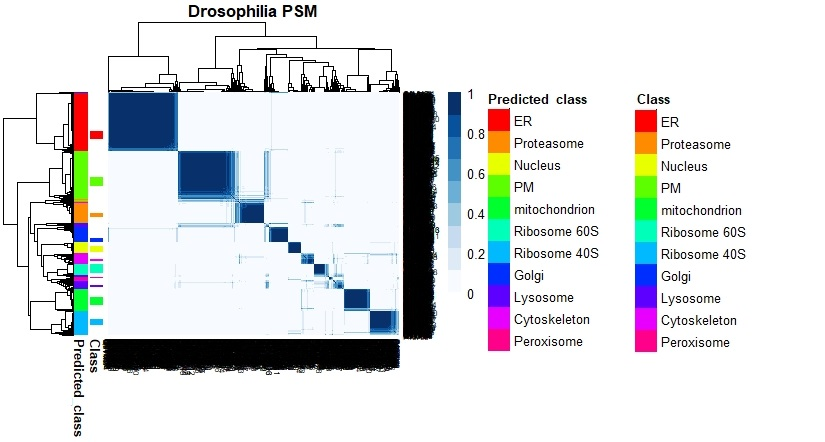
\includegraphics[scale=0.9]{tan_psm_edit}
\caption{Posterior similarity matrix of data from \citet{TanMappingOrganelleProteins2009a}.}
\label{fig:tan_psms}
\end{figure}
To test the robustness of the tagmmdi model, we compare the improvement in prediction compared to the standalone TAGM model under the quadratic loss function. We compare the improvement in prediction from including the GO terms on data from \emph{Arabidopsis} \cite{GroenIdentificationTransGolgiNetwork2014a}, \emph{Drosophila}\cite{TanMappingOrganelleProteins2009a} and mouse stem cells \cite{Christoforoudraftmapmouse2016a}. Within the known proteins we carry out cross validation, holding out $20\%$ of the data as a validation set for 10 separate folds of 15,000 iterations with a burn-in of 5,000. We test for a difference in the variance and mean of the vector of resulting loss values for TAGM and tagmmdi and show them in figure \ref{fig:cv_results}. The results of the tests are shown in table \ref{table:cv_results}.

\begin{figure}[h]
\centering
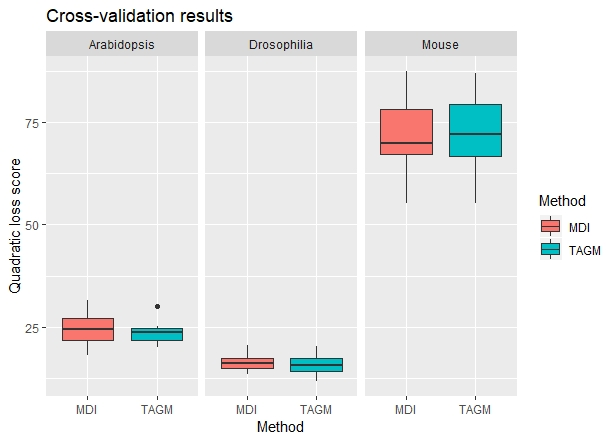
\includegraphics[scale=0.9]{cv_results}
\caption{Boxplot of results of cross-validation.}
\label{fig:cv_results}
\end{figure}
\ctable[
botcap,
%cap = Parameters,
caption = {Results of cross-validation showing $p$-values for tests for difference in mean and variance of loss value for folds for TAGM compared to tagmmdi.},
mincapwidth=12cm,
%label = nowidth,
pos = !htb,
label = table:cv_results
] {lcc} {
}{ \FL
Organism & F-test & t-test \ML
\emph{Arabidopsis} & 0.378 & 0.572 \NN
\emph{Drosophila} & 0.761 & 0.573  \NN
Mouse & 0.861 & 0.947 \LL
}
Based on the lack of significant results we did not apply any multiple test correction \cite{BenjaminiControllingFalseDiscovery1995} as it was deemed unnecessary.

All results were produced using the versions of software and hardware as shown in table \ref{table:hardware}.
\ctable[
botcap,
%cap = Parameters,
caption = {Description of relevant computer hardware and software.},
%mincapwidth=12cm,
%label = nowidth,
pos = !htb,
label = table:hardware
] {ll} {
}{ \FL
Object & Details \ML
Model & LENOVO ideapad 110-17ACL\NN
Processor & AMD A8-7410 APU with AMD Radeon R5 Graphics 2.20 GHz \NN
Available RAM & 6.91GB \NN
OS & Windows 10 Home v 1803 \NN
R version & 3.5.1 \NN
Rstudio version & 1.1.456 \NN
Rcpp version & 0.12.18 \NN
ARMA version & 9.100.5 \LL
}


\section{Conclusions and further work}
Compare to the vanilla TAGM model we see that tagmmdi does significantly differ in table \ref{table:cv_results}. It is worth commenting that there is no disimprovement either, so if the computational cost is not a limit use of tagmmdi models will not offer any risk. We suggest that with a carefully chosen secondary dataset we could acquire information about our subclusters as categorical data is normally more interpretable than continuous data. We state this as the categories are normally human defined whereas continuous data, as a matrix of quantitative measurements, can be slightly dense. This applies less so in the supervised case investigated here, but certainly holds for many unsupervised cases and could reveal information about the subclusters even in the supervised case. We recommend testing the method on different auxiliary datasets such as Protein-Protein Interactions (PPI) to further test its predictive capabilities.

The functions in \emph{tagmmdi} also allow use of a second continuous dataset. This could be used to test the strength of association between replicates or to investigate for new organelles (perhaps by running the second dataset with an unsupervised mixture of Gaussians). The possibility for this later concept is investigated briefly in figure \ref{fig:g_g_psm}.

\begin{figure}[h]
\centering
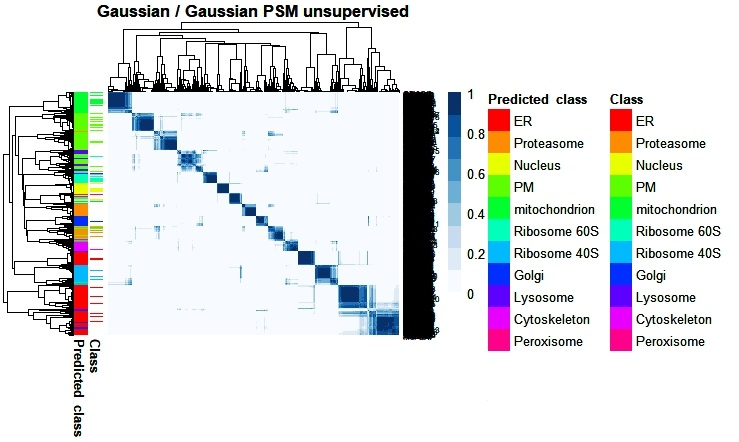
\includegraphics[scale=0.9]{tan_tan_unsupervised_with_prediction_edit}
\caption{Posterior similarity matrix of data from \citet{TanMappingOrganelleProteins2009a} for one dataset with a TAGM model as in figure  \ref{fig:tan_psms} and the second with an over-fitted Gaussian mixture model for which $K=17$. The PSM is for the latter. Class predictions are from the TAGM model.}
\label{fig:g_g_psm}
\end{figure}
One can see that different organelles show strong sub-clusters. This suggests investigating this question and developing extensions to \emph{tagmmdi} for this purpose.

Currently the R package \emph{tagmmdi} is being updated by O. Crook to be integrated into the \emph{Bioconductor} repository as part of the \emph{pRoloc} suite.

Different MCMC methods such as a collapsed Gibbs sampler or Hamiltonian MCMC might lower the computational cost.

\section{Self-reflection}
My main achievements from this internship are:
\begin{itemize}
 \item Learning C++;
 \item Implementing Bayesian analysis; and
 \item Building an R package.
\end{itemize}
Learning C++ was very difficult. I used Armadillo, a linear algebra library, extensively, and it did make the process easier as it is very well documented. However I could not be confident in my coding or know the exact mechanisms of each step, so I needed to compare the version of TAGM in my package to that in \emph{pRoloc}. This is one of the harder things I  have learnt; that for checking your implementation for bugs you just have to do the work. This could be going through the code line by line (which I did several times over the course of the project) or if there is a comparable pre-existing tool recreating results exactly. The latter option was available to me in the form of TAGM models in \emph{pRoloc}, but I did try to avoid the work to make the two directly comparable. Eventually I accepted that I could not move forward without doing it however. To do this a few things were necessary. TAGM uses a collapsed Gibbs sampler and the code is in rather dense R, so I built a C++ version (which produced the same results as that produced by \emph{pRoloc}) and also changed the tagmmdi implementation to a collapsed Gibbs sampler to create results that could be compared before returning to a traditional Gibbs sampler. This allowed me to be sure that there was no bugs in my coding. It was a necessary step, but I avoided it as I hoped there would be an easier alternative. I probably lost a week due to this whereas it really was unavoidable; I hope that from now on I will be quicker to accept that sometimes this kind of work is mandatory. This is the main step I would have changed in this process.

With regards to the inference, I had encountered the concept of the Bayesian paradigm and Bayes' theorem, but actually applying the method to a problem was very difficult. Building the Gibbs sampler and the bookkeeping with all of the components and the various associated vectors and matrices was a difficult and non-intuitive process. However I think that this approach has many strengths and is worth the initial difficulty. The dense output with its uncertainty estimation is very useful and the ability to include expert knowledge in the form of a prior can also be highly beneficial. There are downsides, particularly the computational cost and lack of scalability, to the Bayesian inferential method, so it is worth having as a tool but it also helps to be open-minded and use the correct tool for the correct problem. I am very glad to have had proper exposure to Bayesian inference in general but also to mixture models in particular as they extend to Gaussian and Dirichlet processes, two methods that seem very powerful. With this understanding of the methods implemented, if I was rebuilding the package I think an Object Oriented (OO) implementation of the MDI in C++ is more natural and would make for more concise code.

Building an R package was surprisingly easy thanks to \citet{Wickhampackagesorganizetest2015}. The method is clear and with the RcppArmadillo package one is enabled to setup a package with the correct anatomy to call C++ and Armadillo. This is done by calling:
\begin{lstlisting}
RcppArmadillo.package.skeleton
\end{lstlisting}
At least for me, the package structure encourages better practices with regards to commenting and function writing. I think that it is a very useful way of capturing one's code, and the ease of combining a package with a Github repository via Rstudio is wonderful. I think this is likely to be a key part of my workflow in future.

Overall I am very pleased with what I learnt and what I achieved during the internship. I really enjoyed working with my supervisor Paul Kirk and my time in Cambridge flew past. It was interesting to see the work that the people do there, a lot of it is trial design which I know nothing about. To see the multitude of roles statisticians play in the research of medicine is exciting. I was also lucky enough to be there for the Armitage Day (the MRC Biostatistics Unit's annual seminar), which was pretty nice; Barbara Engelhardt was the keynote speaker. Getting to meet and talk to someone as dynamic as that is quite inspiring. There was a number of smaller scale seminars. I think that due to this exposure, both to more career academics in a social setting (some of the Armitage events were aimed at exposing PhD students to older-hands and I was lucky enough to be included) and to seminars and more varied research, I have a better understanding of what academia is like.

The internship has left me convinced that I want to do a PhD in the future but has left me unsure if long-term academia is suited for me. The unit received its 5-year grant from the MRC in my time there. The work and stress of this grant-hunting seems to be a common feature of an academic's life. This stress of low-security and the high bureaucracy might outweigh the attractions of learning and the freedom of research (relative to industry) in the long term. Fortunately this is not a question I need to answer yet. However I think it helps to enter a PhD with my eyes open and the intention to learn a few skills that are in demand in industry.
\newpage
\appendix

\section{MDI model derivations}
For MDI in the case of $n$ observations in 2 datasets (also referred to as \emph{contexts}):

\begin{align}
p(\left\{c_{i1}, c_{i2}\right\}_{i=1}^n, v) \propto \gamma_{c_{i1}1} \gamma_{c_{i2}2} \left(1 + \phi \mathbb{I}(c_{i1} = c_{i2})\right)  \label{general_model}
\end{align}
We assume priors of $\gamma_{1l},\ldots,\gamma_{nl} \distas{i.i.d} Gamma(\alpha_l/K_l,1)\, \forall \, l \in \{1,2\}$ where $K_l$ is the number of clusters in the $l$th dataset. Similarly $\phi \sim Gamma(a, b)$.

From \eqref{general_model} we calculate the normalising constant $Z$, and find:

\begin{align}
Z = \sum_{k_1=1}^{K_1}\sum_{k_2=1}^{K_2} \gamma_{c_{i1}1} \gamma_{c_{i2}2} \left(1 + \phi \mathbb{I}(k_1 = k_2)\right) \label{normal_const}
\end{align}
The joint density is hence:

\begin{align}
p(\left\{c_{i1}, c_{i2}\right\}_{i=1}^n| \phi) = \frac{1}{Z} \prod_{i = 1}^n  \gamma_{c_{i1}1} \gamma_{c_{i2}2} \left(1 + \phi \mathbb{I}(c_{i1} = c_{i2})\right) \label{joint_density_no_v}
\end{align}
As in \citet{Nieto-BarajasNormalizedrandommeasures2004}, we introduce a strategic latent variable $v$ such that the form is:

\begin{align}
p(\left\{c_{i1}, c_{i2}\right\}_{i=1}^n, v) = \frac{v^{n-1} \exp(-vZ)}{(n-1)!} \prod_{i = 1}^n \left(\left(1 + \phi \mathbb{I}(c_{i1} = c_{i2})\right) \prod_{l = 1}^{2}\gamma_{c_{il}l}\right) \label{joint_density}
\end{align}
Where $Z$ remains as in \eqref{normal_const}.

\subsection{$v$}
From \eqref{joint_density} we can see the conditional for the strategic latent variable $v$ is:

\begin{align}
p(v | \{c_{i1}, c_{i2}\}_{i=1}^n) \propto \frac{v^{n-1}\exp(-vZ)}{(n-1)!}
\end{align}
We recognise this as the pdf for a Gamma distribution with shape $n$ and rate $Z$, i.e. $v \sim Gamma(n, Z)$.

\subsection{$\gamma_{kl}$}
If we expand $Z$ in \eqref{joint_density} we can derive the conditional for the component weights, $\gamma_{kl}$:

\begin{align}
p(\gamma_{kl} | \left\{c_{i1}, c_{i2}\right\}_{i=1}^n) &\propto \exp\left(-v \gamma_{kl} \sum_{k_{l'}=1}^{K_{l'}} \gamma_{c_{il'}l'} \left(1 + \phi \mathbb{I}(k_l = k_{l'})\right)\right) \prod_{i = 1}^n \left(\left(1 + \phi \mathbb{I}(c_{i1} = c_{i2})\right) \prod_{l = 1}^{2}\gamma_{c_{il}l}\right) \mathbb{I}(c_{il} = k) \\
&\propto \exp\left(-v \gamma_{kl} \sum_{k_{l'}=1}^{K_{l'}} \gamma_{c_{il'}l'} \left(1 + \phi \mathbb{I}(k_l = k_{l'})\right)\right) \prod_{i=1}^n \left(1 + \phi \mathbb{I}(c_{i1} = c_{i2})\right) \mathbb{I}(c_{il} = k) \gamma_{kl} \\
& \propto \exp\left(-v \gamma_{kl} \sum_{k_{l'}=1}^{K_{l'}} \gamma_{c_{il'}l'} \left(1 + \phi \mathbb{I}(k_l = k_{l'})\right)\right) \gamma_{kl}^{\sum_{i=1}^n \mathbb{I}(c_{il} = k)}
\end{align}
Where $l' \in \{1,2\} \land l' \neq l$. Thus $\gamma_{kl} \sim Gamma(a_{\gamma}, b_{\gamma})$ where:

\begin{align}
a_{\gamma} &= 1 + \sum_{i=1}^n \mathbb{I}(c_{il} = k) \\
b_{\gamma} &= v \sum_{k_{l'}=1}^{K_{l'}} \gamma_{c_{il'}l'} \left(1 + \phi \mathbb{I}(k_l = k_{l'})\right)
\end{align}

\subsection{$\phi$}
\subsubsection{Conditional probability}
Consider the conditional probability of $\phi$, then from \eqref{joint_density} and expanding $Z$:

\begin{align}
 p(\phi | \left\{c_{i1}, c_{i2}\right\}_{i=1}^n, v) &\propto \exp\left(-v \sum_{k_1=1}^{K_1}\sum_{k_2=1}^{K_2}\left(\left(1 + \phi\mathbb{I}(j_1 = j_2)\right) \prod_{l=1}^2\gamma_{k_ll}\right)\right) \prod_{i = 1}^n \left(\left(1 + \phi \mathbb{I}(c_{i1} = c_{i2})\right) \prod_{l = 1}^{2}\gamma_{c_{il}l}\right) \label{phi_cond_1}
\end{align}
We would like to transform this quantity into a density function we recognise. Consider the two occurrences of $\phi$:

\begin{align}
a &=  \prod_{i = 1}^n \left(\left(1 + \phi \mathbb{I}(c_{i1} = c_{i2})\right) \prod_{l = 1}^{2}\gamma_{c_{il}l}\right)  \label{a} \\
b &=  \sum_{k_1=1}^{K_1}\sum_{k_2=1}^{K_2}\left(\left(1 + \phi\mathbb{I}(k_1 = k_2)\right) \prod_{l=1}^2\gamma_{k_ll}\right) \label{b}
\end{align}
Beginning with \eqref{a}:

\begin{align}
a &= \prod_{i = 1}^n \gamma_{c_{i1}1} \gamma_{c_{i2}2}  \left(1 + \phi \mathbb{I}(c_{i1} = c_{i2})\right) \\
 &= \left(1 + \phi \mathbb{I}(c_{i1} = c_{i2})\right)^n \prod_{i = 1}^n \gamma_{c_{i1}1} \gamma_{c_{i2}2} \\
 &\propto  \left(1 + \phi \mathbb{I}(c_{i1} = c_{i2})\right)^n \\
 &=  \left(1 + \phi)\right)^{\sum_{i=1}^n  \mathbb{I}(c_{i1} = c_{i2})} \\
 &= \sum_{r=0}^{\sum_{i=1}^n  \mathbb{I}(c_{i1} = c_{i2})} \binom{\sum_{i=1}^n  \mathbb{I}(c_{i1} = c_{i2})}{r} \phi^r \qquad (\text{from the binomial theorem})
\end{align}
Here $\sum_{i=1}^n  \mathbb{I}(c_{i1} = c_{i2})$ is the count of observations assigned to the same cluster in both contexts and will be called $c$.

Now consider \eqref{b}:

\begin{align} \label{b_likelihood}
b &=  \sum_{k_1=1}^{K_1}\sum_{k_2=1}^{K_2}\left(\left(1 + \phi\mathbb{I}(k_1 = k_2)\right) \prod_{l=1}^2\gamma_{k_ll}\right)
\end{align}
We see that for our conditional we can ignore all cases when $k_1 \neq k_2$ as $\phi$ is not present in these. Letting $K_{min} = \min(K_1,K_2)$, \eqref{b_likelihood} simplifies to:

\begin{align}
b &\propto \sum_{k=1}^{K_{min}}\gamma_{k1} \gamma_{k2} \left(1 + \phi\right) \\
&\propto \sum_{k=1}^{K_{min}} \gamma_{k1} \gamma_{k2} \phi
\end{align}
Thus updating \eqref{phi_cond_1} accordingly gives us:

\begin{align}
p(\phi | \left\{c_{i1}, c_{i2}\right\}_{i=1}^n, v) &\propto \exp\left(-v \sum_{k=1}^{K_{min}}\gamma_{k1} \gamma_{k2}\phi\right)  \sum_{r=0}^c \binom{c}{r} \phi^r
\end{align}
We notice this has the structure similar to a mixture of Gamma distributions with each distribution having a shape of $r-1$ and a rate of $-v\sum_{k=1}^{K_{min}}\gamma_{k1} \gamma_{k2}$. We thus multiply the equation by 1 to have:

\begin{align}
 p(\left\{c_{i1}, c_{i2}\right\}_{i=1}^n, v | \phi) &\propto  \sum_{r=0}^c \binom{c}{r} \frac{r!}{\left(v \sum_{k=1}^{K_{min}} \gamma_{k1} \gamma_{k2}\right)^{r+1}}  \frac{\left(v \sum_{k=1}^{K_{min}} \gamma_{k1} \gamma_{k2}\right)^{r+1}}{r!}\phi^r \exp\left(-v \sum_{k=1}^{K_{min}} \gamma_{k1} \gamma_{k2}\phi\right) \\
&= \sum_{r=0}^c  \binom{c}{r} \frac{r!}{\left(v \sum_{k=1}^{K_{min}} \gamma_{k1} \gamma_{k2}\right)^{r+1}} Gamma\left(r+1, v \sum_{k=1}^{K_{min}} \gamma_{k1} \gamma_{k2} \right)
\end{align}
As we know that $p(\phi | \left\{c_{i1}, c_{i2}\right\}_{i=1}^n, v)$ must integrate over $\phi$ to 1, we know the normalising constant must be the sum of the integrals of the Gamma distributions, i.e.:

\begin{align}
Z_{\phi} &= \sum_{r=0}^c   \binom{c}{r} \frac{r!}{\left(v \sum_{k=1}^{K_{min}} \gamma_{k1} \gamma_{k2}\right)^{r+1}}  \int\frac{\left(v \sum_{k=1}^{K_{min}} \gamma_{k1} \gamma_{k2}\right)^{r+1}}{r!}\phi^r \exp\left(-v \sum_{k=1}^{K_{min}} \gamma_{k1} \gamma_{k2}\phi\right) d\phi \\
&= \sum_{r=0}^c  \binom{c}{r} \frac{r!}{\left(v \sum_{k=1}^{K_{min}} \gamma_{k1} \gamma_{k2}\right)^{r+1}}  \label{Z_phi}
\end{align}
Combining these gives:

\begin{align}
p(\phi | \left\{c_{i1}, c_{i2}\right\}_{i=1}^n, v) &= \frac{1}{Z_{\phi}}  \sum_{r=0}^c  \binom{c}{r} \frac{r!}{\left(v \sum_{k=1}^{K_{min}} \gamma_{k1} \gamma_{k2}\right)^{r+1}} Gamma\left(r+1, v \sum_{k=1}^{K_{min}} \gamma_{k1} \gamma_{k2} \right)
\end{align}

\subsubsection{Posterior distribution}

Now if we consider a prior of $Gamma(a_0, b_0)$ on the $\phi$, we have a prior probability of:

\begin{align}
p(\phi) &= \frac{b_0^{a_0}}{(a_0 - 1)!}\phi^{a_0 - 1}\exp\left(-b_0 \phi \right)
\end{align}
Thus our posterior conditional is:

%  \frac{r!}{\left(v \sum_{k=1}^{K_{min}} \gamma_{k1} \gamma_{k2}\right)^{r+1}}  \frac{\left(v \sum_{k=1}^{K_{min}} \gamma_{k1} \gamma_{k2}\right)^{r+1}}{r!}

\begin{align}
p(\phi | \cdot) &\propto p(\phi) p(\left\{c_{i1}, c_{i2}\right\}_{i=1}^n, v | \phi)  \\
&\propto \frac{b_0^{a_0}}{(a_0 - 1)!}\phi^{a_0 - 1}\exp\left(-b_0 \phi \right)  \sum_{r=0}^c  \binom{c}{r}\phi^r \exp\left(-v \sum_{k=1}^{K_{min}} \gamma_{k1} \gamma_{k2}\phi\right) \\
&\propto \sum_{r=0}^c  \binom{c}{r} \phi^{r + a_0 - 1} \exp \left( \left(-v \sum_{k=1}^{K_{min}} \gamma_{k1} \gamma_{k2}  -b_0 \right)\phi\right)
\end{align}
We now use the same trick as with the likelihood to move towards the shape of a Gamma density function, and multiply by 1:

\begin{align}
\nonumber p(\phi | \cdot) &\propto & \sum_{r=0}^c  \binom{c}{r} \frac{(r + a_0 - 1)!}{ \left(v \sum_{k=1}^{K_{min}} \gamma_{k1} \gamma_{k2} + b_0 \right)^{r + a_0}} \times & \\
& &\frac{ \left(v \sum_{k=1}^{K_{min}} \gamma_{k1} \gamma_{k2} + b_0 \right)^{r + a_0}}{(r + a_0 - 1)!} \phi^{r + a_0 - 1} & \exp \left( - \left(v \sum_{k=1}^{K_{min}} \gamma_{k1} \gamma_{k2} + b_0 \right)\phi\right)
\end{align}
We recognise the rightmost terms as the pdf of a Gamma distribution with shape $r + \alpha_0$ and rate $v\sum_{k=1}^{K_{min}}\gamma_{k1}\gamma_{k2} + b_0$. Thus:
\begin{align}
p(\phi | \cdot) &\propto \sum_{r=0}^c  \binom{c}{r} \frac{(r + a_0 - 1)!}{ \left(v \sum_{k=1}^{K_{min}} \gamma_{k1} \gamma_{k2} + b_0 \right)^{r + a_0}} Gamma \left(r+ a_0, v \sum_{k=1}^{K_{min}} \gamma_{k1} \gamma_{k2} + b_0 \right)
\end{align}
Again we have a mixture of Gamma densities. For the normalising constant we have an expression similar to \eqref{Z_phi}:

\begin{align}
\nonumber Z_{\phi}' &=& \sum_{r=0}^c  \binom{c}{r} \frac{(r + a_0 - 1)!}{ \left(v \sum_{k=1}^{K_{min}} \gamma_{k1} \gamma_{k2} + b_0 \right)^{r + a_0}} \times & \\
&& \int \frac{ \left(v \sum_{k=1}^{K_{min}} \gamma_{k1} \gamma_{k2} + b_0 \right)^{r + a_0}}{(r + a_0 - 1)!} \phi^{r + a_0 - 1} & \exp \left( - \left(v \sum_{k=1}^{K_{min}} \gamma_{k1} \gamma_{k2} + b_0 \right)\phi\right) d\phi_{12}
\end{align}
We recognise the integral as the pdf of a Gamma distribution and know it must integrate to 1. This leaves:

\begin{align}
Z_{\phi}' &= \sum_{r=0}^c \binom{c}{r} \frac{(r + a_0 - 1)!}{ \left(v \sum_{k=1}^{K_{min}} \gamma_{k1} \gamma_{k2} + b_0 \right)^{r + a_0}} 
\end{align}
Thus the posterior distribution of the context similarity parameter $\phi$ is:

\begin{align}
p(\phi |  \left\{c_{i1}, c_{i2}\right\}_{i=1}^n, v) &=  \frac{1}{Z_{\phi}'} \sum_{r=0}^c  \binom{c}{r} \frac{(r + a_0 - 1)!}{ \left(v \sum_{k=1}^{K_{min}} \gamma_{k1} \gamma_{k2} + b_0 \right)^{r + a_0}} Gamma \left(r+ a_0, v \sum_{k=1}^{K_{min}} \gamma_{k1} \gamma_{k2} + b_0 \right)
\end{align}

\newpage
\section*{Acknowledgments}
Thanks are due to my supervisors Paul Kirk (primary) and Laurent Gatto (secondary) as well as their PhD student Oliver M Crook who was very free with his time in explaining concepts to me. The project was designed and overseen by Paul who also took the time to run through my code on a few occasions which is an intimidating task for the unwary. All the people at the MRC Biostatistics Unit, Cambridge University made my stay there very pleasant as well as educational.

Thanks also to Aalt-Jan van Dijk for agreeing to supervise me from Wageningen thereby enabling this project.

With regards to software this project was massively enabled by RStudio \cite{RStudioTeamRStudioIntegratedDevelopment2016} and GitHub. \citet{EddelbuettelRcppSeamlessIntegration2011} deserve special mention for the development of Rcpp which made integrating the Gibbs sampler from C++ far easier. The C++ is almost entirely coded using objects and functions from Armadillo \cite{SandersonArmadillotemplatebasedlibrary2016}.

The advice from \citet{BryanExcusemeyou} was much appreciated and saved an awful lot of time. 

\newpage
%\bibliographystyle{abbrv}
\bibliographystyle{plainnat}
\bibliography{tagmmdi_literature}

\end{document}

